\documentclass[a4paper,12pt,titlepage]{article}



\usepackage{index}
\makeindex
\usepackage[a4paper, inner=0.5cm, outer=1.5cm, top=2cm, bottom=2cm, bindingoffset=1.2cm]{geometry}
\usepackage[english]{babel}

% define my own color
\usepackage{xcolor}
\definecolor{comment}{RGB}{120,120,120}
\definecolor{codenumber}{RGB}{100,100,100}
\definecolor{shade}{RGB}{220,220,220}
\definecolor{link}{RGB}{0,0,225}
\definecolor{url}{RGB}{30,144,255}

\usepackage{framed}
\usepackage{graphicx}
\usepackage{wrapfig}
\usepackage{blindtext}

%make the section title centered
\usepackage{sectsty}
\sectionfont{\centering}

\usepackage{enumitem}


% use font package
\usepackage{fontspec}
% change the font
\setmonofont{Menlo}


% provides different line thicknesses for tables
\usepackage{booktabs}

%prevents figures ever floating backwards up the current page
\usepackage{flafter}

% here for H placement parameter
\usepackage{float} 

\usepackage{makecell, caption}

% enable inserting codes
\usepackage{listings}

\lstset{
  language={Java},
  commentstyle=\color{comment},
  basicstyle=\footnotesize\ttfamily,
  numbers=left,
  numberstyle=\scriptsize\color{codenumber},
  frame=single,		% add the frame
  breaklines=true,	% sets automatic line breaking
 % texcsstyle=*\color{red},
 % identifierstyle=\color{magenta},
  extendedchars,
  escapeinside=``,	% used for escaping
  tabsize=2
}

\lstset{
  literate=*{¡\\!}{{\textcolor{red}{\textbackslash!}}}{2}
            {¡\\"}{{\textcolor{red}{\textbackslash"}}}{2}
            {¡\\\#}{{\textcolor{red}{\textbackslash\#}}}{2}
            {¡\\\$}{{\textcolor{red}{\textbackslash\$}}}{2}
            {¡\\\%}{{\textcolor{red}{\textbackslash\%}}}{2}
            {¡\\\&}{{\textcolor{red}{\textbackslash\&}}}{2}
            {¡\\'}{{\textcolor{red}{\textbackslash'}}}{2}
            {¡\\(}{{\textcolor{red}{\textbackslash(}}}{2}
            {¡\\)}{{\textcolor{red}{\textbackslash)}}}{2}
            {¡\\*}{{\textcolor{red}{\textbackslash*}}}{2}
            {¡\\+}{{\textcolor{red}{\textbackslash+}}}{2}
            {¡\\,}{{\textcolor{red}{\textbackslash,}}}{2}
            {¡\\-}{{\textcolor{red}{\textbackslash-}}}{2}
            {¡\\.}{{\textcolor{red}{\textbackslash.}}}{2}
            {¡\\/}{{\textcolor{red}{\textbackslash/}}}{2}
            {¡\\:}{{\textcolor{red}{\textbackslash:}}}{2}
            {¡\\;}{{\textcolor{red}{\textbackslash;}}}{2}
            {¡\\<}{{\textcolor{red}{\textbackslash<}}}{2}
            {¡\\=}{{\textcolor{red}{\textbackslash=}}}{2}
            {¡\\>}{{\textcolor{red}{\textbackslash>}}}{2}
            {¡\\?}{{\textcolor{red}{\textbackslash?}}}{2}
            {¡\\[}{{\textcolor{red}{\textbackslash[}}}{2}
            {¡\\\\}{{\textcolor{red}{\textbackslash\textbackslash}}}{2}
            {¡\\]}{{\textcolor{red}{\textbackslash]}}}{2}
            {¡\\\^}{{\textcolor{red}{\textbackslash\textasciicircum}}}{2}
            {¡\\\{}{{\textcolor{red}{\textbackslash\{}}}{2}
            {¡\\|}{{\textcolor{red}{\textbackslash|}}}{2}
            {¡\\\}}{{\textcolor{red}{\textbackslash\}}}}{2}
            {¡\\\~}{{\textcolor{red}{\textbackslash\textasciitilde}}}{2}
}

% E.g.
% \begin{lstlisting}
% ¡\! ¡\" ¡\# ¡\$ ¡\% ¡\& ¡\' ¡\( ¡\) ¡\* ¡\+ ¡\, ¡\- ¡\. ¡\/ ¡\: ¡\; ¡\< ¡\= ¡\> ¡\? ¡\[ ¡\\ ¡\] ¡\^ ¡\{ ¡\| ¡\} ¡\~
% \end{lstlisting}



% Use hyperlink
\usepackage{hyperref}


\urlstyle{sf}

\hypersetup{
    colorlinks=true,
    linkcolor=link,
    filecolor=magenta,      
    urlcolor=cyan,
}


% For math formulas
\usepackage{amsmath}




% documents begins here
\begin{document}

\title{\Large{\textbf{Description of 4302 Example Program}}}
\author{By Xiang Chen (Echo)}
\date{Feb 7, 2020}
\maketitle
\tableofcontents
\newpage

%%%%%%%%%%%%%%%%%%%%%%%%%%%%%%%%%%%%%%%%%%%%%%%%%%%%%%%
%%%%%%%%%%%%%%%%%%%%%%%%%%%%%%%%%%%%%%%%%%%%%%%%%%%%%%%
% Alias
%%%%%%%%%%%%%%%%%%%%%%%%%%%%%%%%%%%%%%%%%%%%%%%%%%%%%%%
%%%%%%%%%%%%%%%%%%%%%%%%%%%%%%%%%%%%%%%%%%%%%%%%%%%%%%%
\section {Alias}
In this description, I will use two alias:
\begin{lstlisting}
alias antlr4='java -jar /usr/local/lib/antlr-4.7.2-complete.jar'

alias grun='java org.antlr.v4.gui.TestRig'
\end{lstlisting}
~\\
Where {\bf antlr4} will be used to run the Antlr complete JAR file (the path will be the location where you put your Antlr JAR file), and {\bf grun} will be used to run the Antlr build-in TestRig for testing the grammar.

%%%%%%%%%%%%%%%%%%%%%%%%%%%%%%%%%%%%%%%%%%%%%%%%%%%%%%%
%%%%%%%%%%%%%%%%%%%%%%%%%%%%%%%%%%%%%%%%%%%%%%%%%%%%%%%
% Visitor version
%%%%%%%%%%%%%%%%%%%%%%%%%%%%%%%%%%%%%%%%%%%%%%%%%%%%%%%
%%%%%%%%%%%%%%%%%%%%%%%%%%%%%%%%%%%%%%%%%%%%%%%%%%%%%%%
\section{Visitor Version}
Antlr 4 has a build-in visitor pattern for transforming Antlr AST into whatever structure you want. Here I create my own structure for the expression hierarchy.
\\
\\
Below is the overall structure of the whole program:
\begin{figure}[H]
\centering
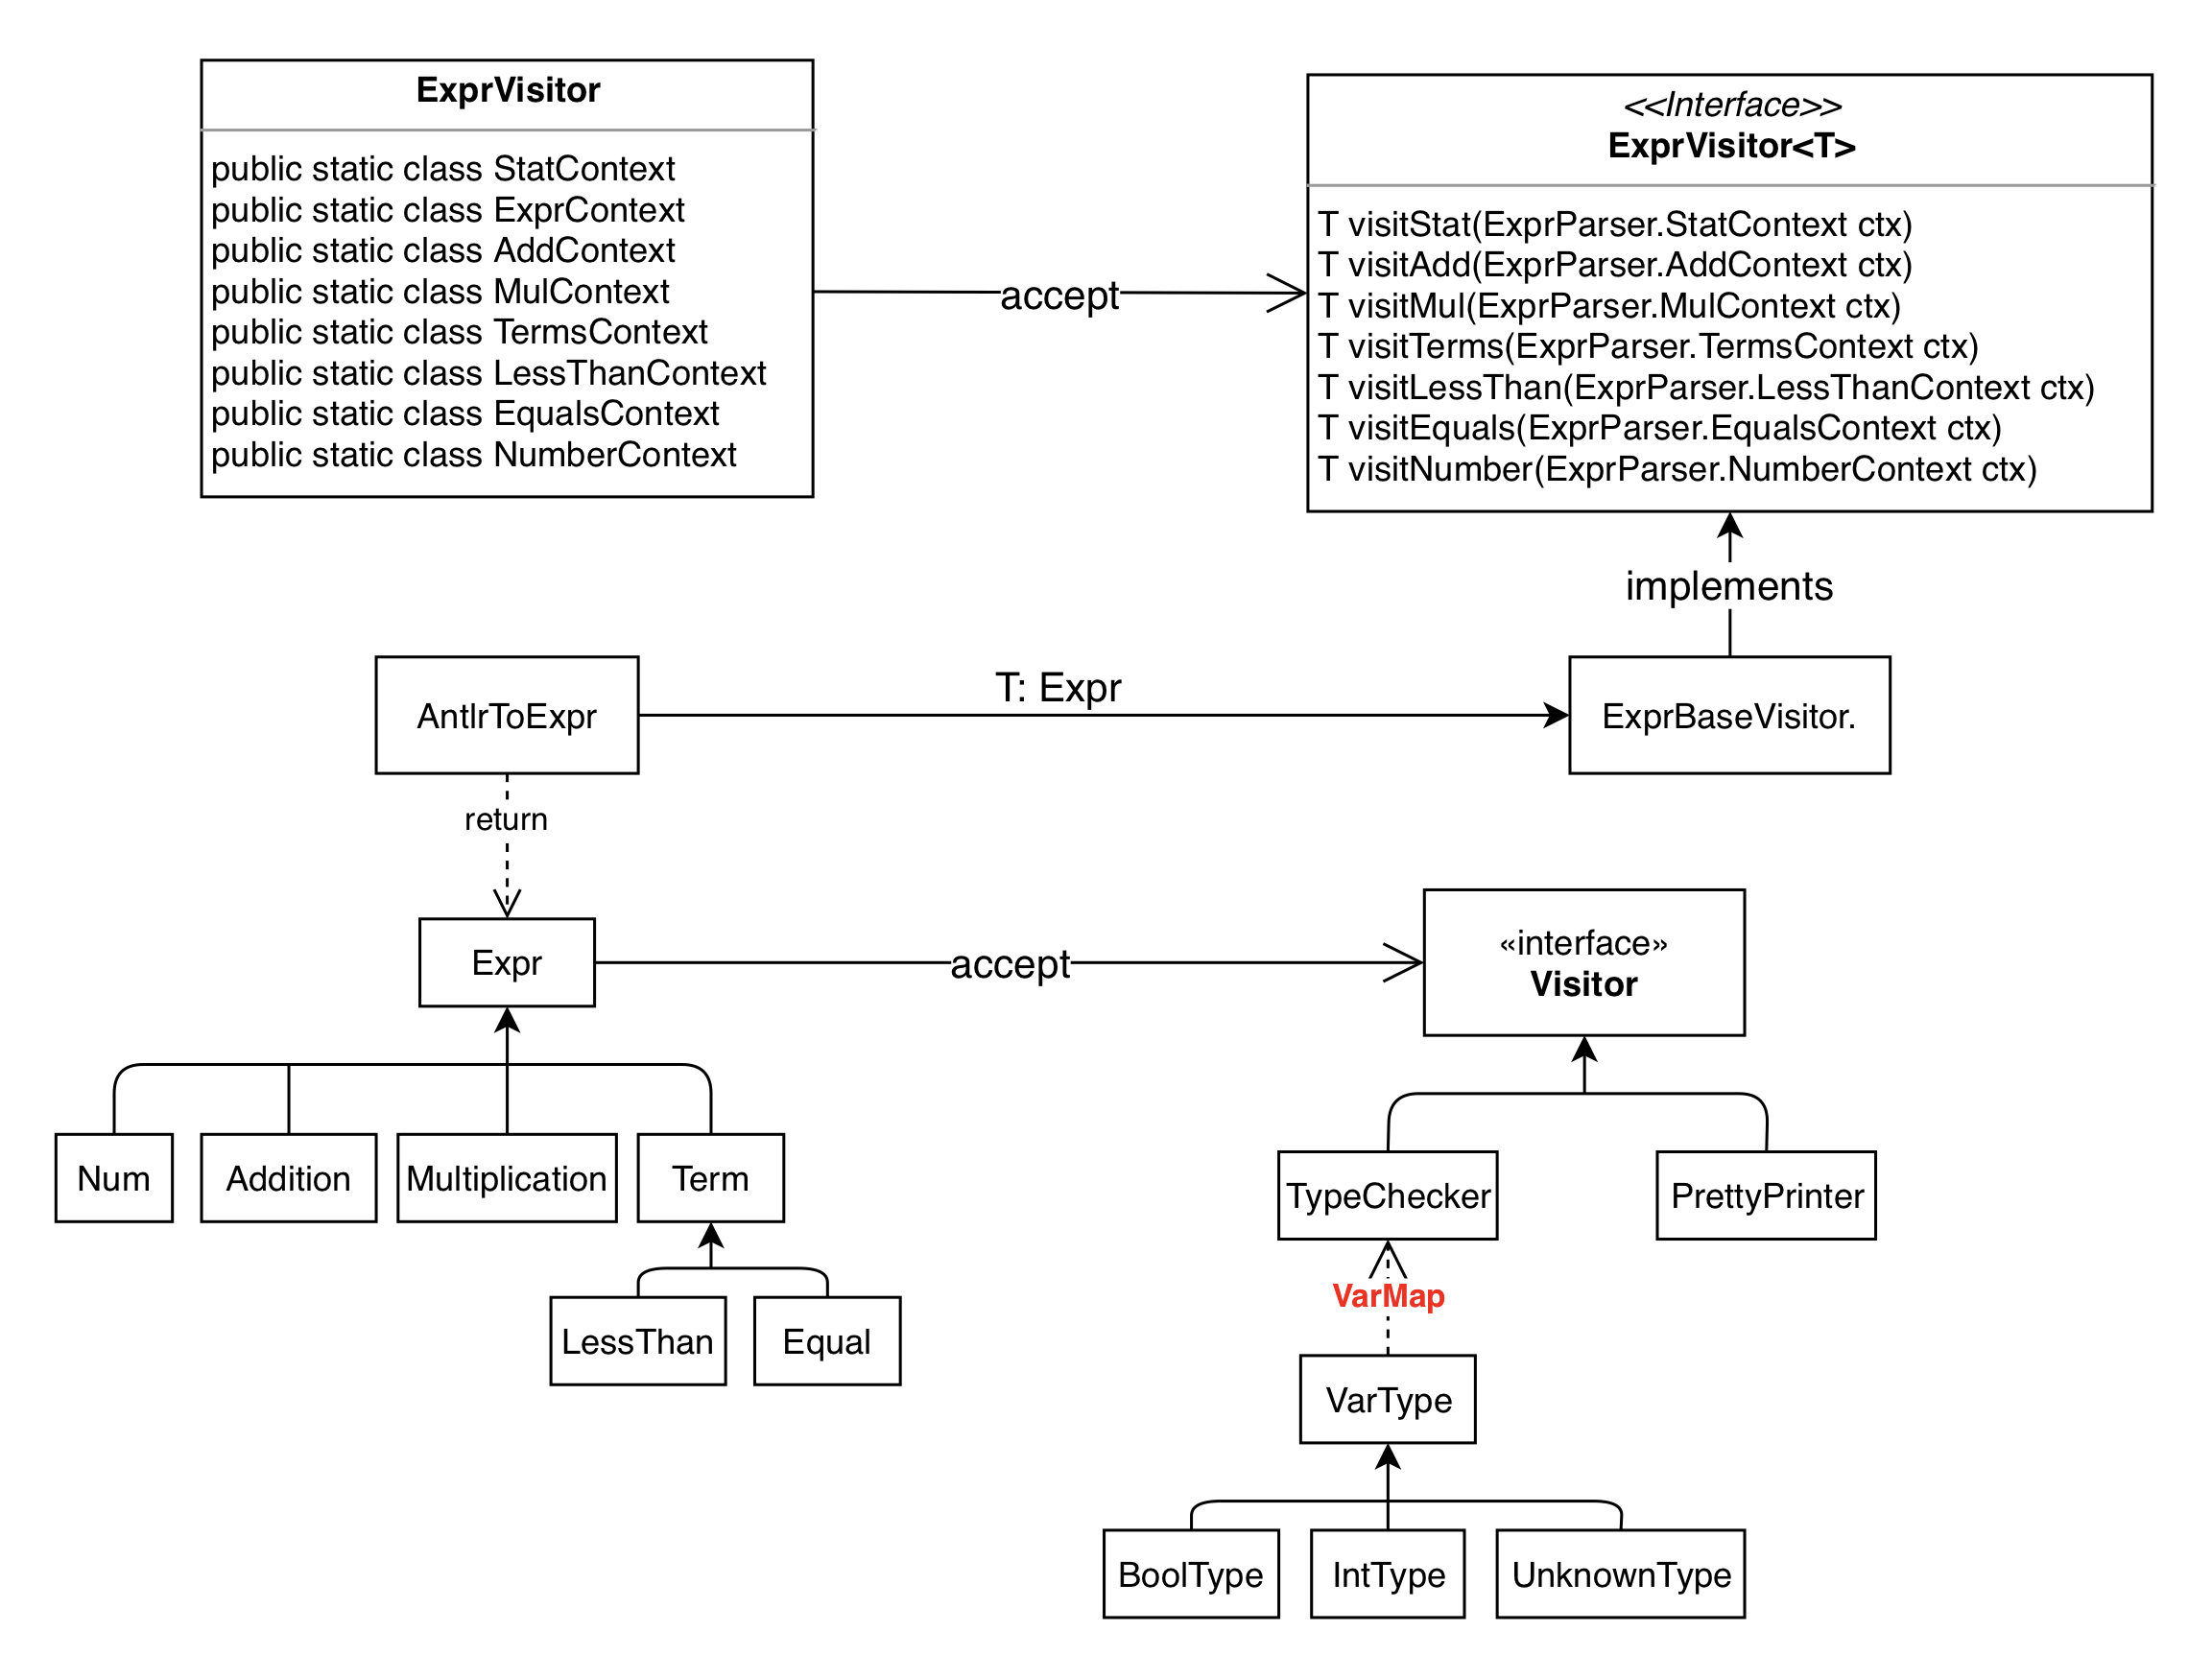
\includegraphics[width=\linewidth]{4302visitor.jpg}
\end{figure}

%%%%%%%%%%%%%%%%%%%%%%%%%%%%%%%%%%%%%%%%%%%%%%%%%%%%%%%
% Steps of Compiling the grammar file
%%%%%%%%%%%%%%%%%%%%%%%%%%%%%%%%%%%%%%%%%%%%%%%%%%%%%%%
\subsection{Steps of Compiling the Grammar File}
Below are the steps of compiling the grammar file for future modification, such as creating our own Expr hierarchy:
\begin{enumerate}
  \item {\footnotesize\ttfamily antlr4 -visitor Expr.g4} \\
  	This step will compile the grammar file. Remember to add the {\footnotesize\ttfamily -visitor} argument, it will automatically generate the necessary classes for the Antlr build-in visitor pattern.
	\item {\footnotesize\ttfamily javac Expr*.java} \\
	This step will compile all the Java files that generated by Antlr. \\
	After this step, you could feel free to import everything into Eclipse and create your own Expr hierarchy and other necessary classes.
	\item {\footnotesize\ttfamily grun Expr stat -gui test01.txt} \\
	This extra step could be used to test if the input file is consistent with the grammar. It will call the Antlr build-in TestRig for testing.
	The {-gui} argument will generate a figure for the Antlr parse tree of user input. Below is an example:
		\begin{figure}[H]
		\centering
		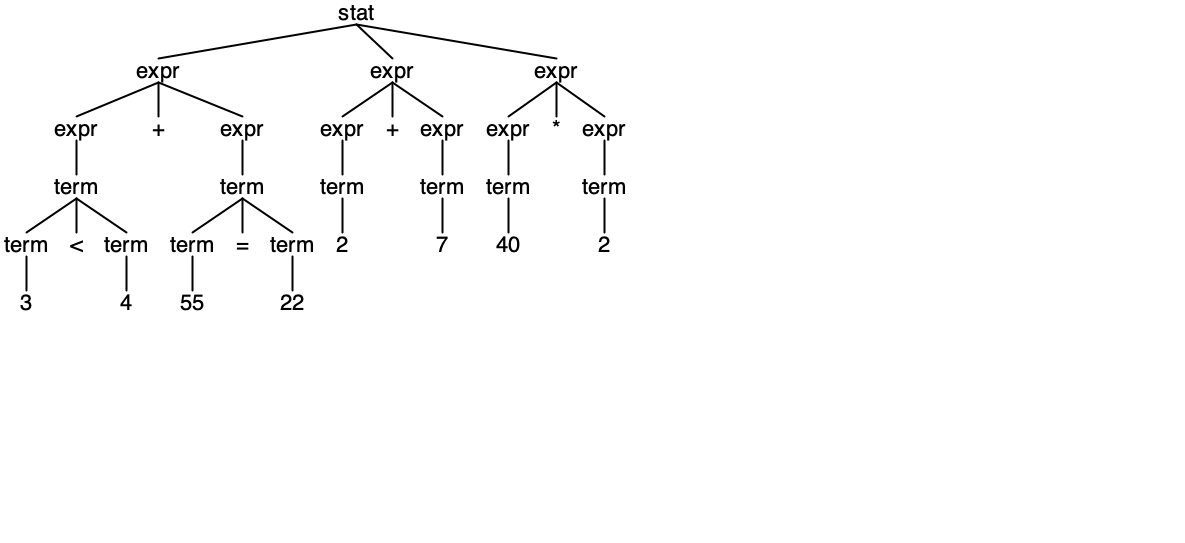
\includegraphics[width=\linewidth]{antlr4_parse_tree.png}
		\end{figure}
\end{enumerate}




%%%%%%%%%%%%%%%%%%%%%%%%%%%%%%%%%%%%%%%%%%%%%%%%%%%%%%%
% Grammar
%%%%%%%%%%%%%%%%%%%%%%%%%%%%%%%%%%%%%%%%%%%%%%%%%%%%%%%
\subsection{Grammar}
The grammar is called {\footnotesize\ttfamily Expr}, and the grammar file will have the extension of {\bf .g4}, also the file name should have the same name as the grammar name.
\\
\\
Below is the grammar:
\begin{lstlisting}
grammar Expr;
// this is the start symbol
stat : expr+;


expr
	: expr MUL expr 			# Mul
	| expr ADD expr 			# Add
	| term 								# Terms
	;


term
	: term LESSTHAN term 		# LessThan
	| term EQUAL term 			# Equals
	| NUM 									# Number
	;


ADD : '+';
MUL : '*';
EQUAL : '=';
LESSTHAN : '<';


NUM : '0'|'-'?[1-9][0-9]*;


COMMENT : '--' ~[\r\n]* -> skip;
WS  :   [ \t\n]+ -> skip ;
\end{lstlisting}
~\\

%%%%%%%%%%%%%%%%%%%%%%%%%%%%%%%%%%%%%%%%%%%%%%%%%%%%%%%
% Explaination
%%%%%%%%%%%%%%%%%%%%%%%%%%%%%%%%%%%%%%%%%%%%%%%%%%%%%%%
\subsection{Explaination}
\begin{itemize}
  	\item Those {\bf labels} are used for generating Antlr build-in visitor methods.
  	\item For example, if you use the label {\footnotesize\ttfamily \#Mul}, Antlr will automatically generate the method called {\footnotesize\ttfamily visitMul()} in the class {\footnotesize\ttfamily ExprBaseVisitor<T>} and interface {\footnotesize\ttfamily ExprVisitor<T>}.
	\item Then you can create your own class, let it inherit the {\footnotesize\ttfamily ExprBaseVisitor<T>} class, and set the generic parameter as what you want, ane rewrite those methods.
	\item Here I create my own class called {\footnotesize\ttfamily AntlrToExpr}, set up the generic parameter as {\footnotesize\ttfamily Expr} and rewrite the necessary methods.
\end{itemize}
~\\

%%%%%%%%%%%%%%%%%%%%%%%%%%%%%%%%%%%%%%%%%%%%%%%%%%%%%%%
% Intermediate Class: AntlrToExpr
%%%%%%%%%%%%%%%%%%%%%%%%%%%%%%%%%%%%%%%%%%%%%%%%%%%%%%%

\subsection{Intermediate Class: AntlrToExpr}
This intermediate class will transform the Antlr AST into my Expr object.
\\
\\
\\
Below is the code for my  {\footnotesize\ttfamily AntlrToExpr} class:
\begin{lstlisting}
package expr;

import antlr.*;
import antlr.ExprParser.*;
import expr.composite.*;

public class AntlrToExpr extends ExprBaseVisitor<Expr>{
	
	
	@Override
	public Expr visitAdd(AddContext ctx) {
		return new Addition(visit(ctx.expr(0)), visit(ctx.expr(1))); 
	}
	
	@Override
	public Expr visitMul(MulContext ctx) {
		return new Multiplication(visit(ctx.expr(0)), visit(ctx.expr(1))); 
	}
	
	@Override
	public Expr visitTerms(TermsContext ctx) {
		return visit(ctx.term());
	}
	
	@Override
	public Expr visitLessThan(LessThanContext ctx) {
		return new LessThan(visit(ctx.term(0)), visit(ctx.term(1))); 
	}
	
	@Override
	public Expr visitEquals(EqualsContext ctx) {
		return new Equal(visit(ctx.term(0)), visit(ctx.term(1))); 
	}
	
	@Override
	public Expr visitNumber(NumberContext ctx) {
		return new Num(ctx.NUM().getText());
	}
}
\end{lstlisting}

\begin{itemize}
	\item Here I set up the generic parameter as {\footnotesize\ttfamily Expr}, so every method in the class will return an Expr object, then I'll call my {\footnotesize\ttfamily TypeChecker} class to traverse the Expr object.
  	\item In the grammar, each of {\footnotesize\ttfamily expr MUL expr, expr ADD expr} contains two {\footnotesize\ttfamily expr} rules, we could refer to them as {\footnotesize\ttfamily expr(0)} and {\footnotesize\ttfamily expr(1)}.
	\item Similarly, each of {\footnotesize\ttfamily term LESSTHAN term, term EQUAL term} contains two {\footnotesize\ttfamily term} rules, we could refer to them as {\footnotesize\ttfamily term0} and {\footnotesize\ttfamily term(1)}.
	\item For the method {\footnotesize\ttfamily visitNumber}, this rule contains one Lexer rule called {\footnotesize\ttfamily NUM}, then we could call this rule by {\footnotesize\ttfamily ctx.NUM()} directly, and {\footnotesize\ttfamily getText()} method will return the String of the Lexer rule NUM.
\end{itemize}
~\\

%%%%%%%%%%%%%%%%%%%%%%%%%%%%%%%%%%%%%%%%%%%%%%%%%%%%%%%
% TypeCheker and PrettyPrinter
%%%%%%%%%%%%%%%%%%%%%%%%%%%%%%%%%%%%%%%%%%%%%%%%%%%%%%%
\subsection{TypeCheker and PrettyPrinter}

\subsubsection{TypeCheker}
The most important part in the Typecheker class is the symbol table called  {\footnotesize\ttfamily varMap}, which helps to check the type for every small expression and constant.
\\
\\
Below is the code for my  {\footnotesize\ttfamily TypeCheker} class:
\begin{lstlisting}
package expr.visitor;

import expr.composite.*;
import java.util.*;
import types.*;

public class TypeChecker implements Visitor{
	// hashmap for type checking
	public static Map<String, VarType> varMap =  new HashMap<String, VarType>();
	
	// error message
	public List<String> errormsg;
	
	// constructor
	public TypeChecker() {
		errormsg = new ArrayList<String>();
	}
	
	// type checker for binary relational expr
	// e.g. =, >, <, >=, <=
	public void relationalBinaryChecker(Expr e) {
		TypeChecker leftChecker = new TypeChecker();
		TypeChecker rightChecker = new TypeChecker();
		
		e.left().accept(leftChecker);
		e.right().accept(rightChecker);
		
		PrettyPrinter leftPrinter = new PrettyPrinter();
		PrettyPrinter rightPrinter = new PrettyPrinter();
		
		e.left().accept(leftPrinter);
		e.right().accept(rightPrinter);
		
		PrettyPrinter printer = new PrettyPrinter();
		e.accept(printer);
		
		errormsg.addAll(leftChecker.errormsg);
		errormsg.addAll(rightChecker.errormsg);
		
		// if left child is not int type of real type
		if (!(varMap.get(leftPrinter.output) instanceof types.IntType)) {
			varMap.put(leftPrinter.output, new UnknowType());
			errormsg.add(leftPrinter.output + " is not integer type. " 
					+ printer.output + " is not type correct.");
			
		}
		
		// if right child is not int type of real type
		if (!(varMap.get(rightPrinter.output) instanceof types.IntType)) {
			varMap.put(rightPrinter.output, new UnknowType());
			errormsg.add(rightPrinter.output + " is not integer type. "
					+ printer.output + " is not type correct.");
		}
		
		// if left and right child are both arithmetic type (no type error)
		// add this expr to the varmap
		varMap.put(printer.output, new BoolType());
	}
	
	// type checker for binary arithmetic expr
	// e.g. +, -, *, /
	public void arithmeticBinaryChecker(Expr e) {
		TypeChecker leftChecker = new TypeChecker();
		TypeChecker rightChecker = new TypeChecker();
		
		e.left().accept(leftChecker);
		e.right().accept(rightChecker);
		
		PrettyPrinter leftPrinter = new PrettyPrinter();
		PrettyPrinter rightPrinter = new PrettyPrinter();
		
		e.left().accept(leftPrinter);
		e.right().accept(rightPrinter);
		
		PrettyPrinter printer = new PrettyPrinter();
		e.accept(printer);
		
		errormsg.addAll(leftChecker.errormsg);
		errormsg.addAll(rightChecker.errormsg);
		
		// if left child is not int type 
		if (!(varMap.get(leftPrinter.output) instanceof types.IntType)) {
			
			varMap.put(leftPrinter.output, new UnknowType());
			errormsg.add(leftPrinter.output + " is not integer type. " 
					+ printer.output + " is not type correct.");
		}
			
		// if right child is not int type or real type
		if (!(varMap.get(rightPrinter.output) instanceof types.IntType)) {
			
			varMap.put(rightPrinter.output, new UnknowType());
			errormsg.add(rightPrinter.output + " is not integer type. "
					+ printer.output + " is not type correct.");
		}
		
		// if both left and right child are int type, the whole expr will be int type
			varMap.put(printer.output, new IntType());
	}
	
	// arithmetic equal (==)
	@Override
	public void visitEqual(Equal e) {
		relationalBinaryChecker(e);
	}

	// arithmetic greater than (>)
	@Override
	public void visitLessThan(LessThan e) {
		relationalBinaryChecker(e);
	}

	// arithmetic add (+)
	@Override
	public void visitAddition(Addition e) {
		arithmeticBinaryChecker(e);
	}

	// arithmetic multiply (*)
	@Override
	public void visitMultiplication(Multiplication e) {
		arithmeticBinaryChecker(e);
	}

	// int number constant
	@Override
	public void visitNum(Num c) {
		if (!varMap.containsKey(c.name)) {
			varMap.put(c.name, new IntType());
		}
	}
}
\end{lstlisting}

\begin{itemize}
	\item This class is very simple, for binary expression, just recursively check if its left child and right child are type correct. If anyone of them is not type correct, then output the error message.
	\item For the base case, which is constant number, it is always type correct.
\end{itemize}
~\\

\subsubsection{PrettyPrinter}
The {\footnotesize\ttfamily PrettyPrinter} class will format the user input, then we could use it to output the error message in the TypeChecker class.
\\
\\
Below is the code for my  {\footnotesize\ttfamily PrettyPrinter} class:
\begin{lstlisting}
package expr.visitor;

import expr.composite.*;

public class PrettyPrinter implements Visitor{
	
	public String output;
	
	public PrettyPrinter() {
		output = "";
	}
	
	public void visitBinaryExpr (Expr b, String op) {
		PrettyPrinter leftPrinter = new PrettyPrinter();
		PrettyPrinter rightPrinter = new PrettyPrinter();
		
		b.left().accept(leftPrinter);
		b.right().accept(rightPrinter);
		output = output.concat("(" + leftPrinter.output 
			+ " " + op + " " + rightPrinter.output + ")");
	}
	
	@Override
	public void visitEqual(Equal e) {
		visitBinaryExpr(e, "=");
	}

	@Override
	public void visitLessThan(LessThan e) {
		visitBinaryExpr(e, "<");
	}

	@Override
	public void visitAddition(Addition e) {
		visitBinaryExpr(e, "+");
	}

	@Override
	public void visitMultiplication(Multiplication e) {
		visitBinaryExpr(e, "*");
	}
	
	@Override
	public void visitNum(Num c) {
		output = output.concat(c.name);	
	}
}
\end{lstlisting}

%%%%%%%%%%%%%%%%%%%%%%%%%%%%%%%%%%%%%%%%%%%%%%%%%%%%%%%
% Main Test Class: TestExpr
%%%%%%%%%%%%%%%%%%%%%%%%%%%%%%%%%%%%%%%%%%%%%%%%%%%%%%%
\subsection{Main Test Class: TestExpr}
This class contains the Main class, and we could use it to parse the user input and run the program.
\\
\\
Below is the code for my  {\footnotesize\ttfamily TestExpr} class:
\begin{lstlisting}
package root;

import org.antlr.v4.runtime.*;
import org.antlr.v4.runtime.tree.*;
import java.io.*;
import java.util.*;
import antlr.*;
import expr.*;
import expr.composite.*;
import expr.visitor.*;

public class TestExpr {
	
	public static void main(String[] args) {
		
		try {
			String inputFile = null;
	        if ( args.length>0 ) 
	        	inputFile = args[0];
	        
	        InputStream is = System.in;
	        
	        if ( inputFile!=null ) {
	            is = new FileInputStream(inputFile);
	        }
	        
	        // parse the input
			ANTLRInputStream input = new ANTLRInputStream(is);
			ExprLexer lexer = new ExprLexer(input);
			CommonTokenStream tokens = new CommonTokenStream(lexer);			
			ExprParser parser = new ExprParser(tokens);
	       
			// tell ANTLR to build a parse tree
			parser.setBuildParseTree(true);
			// parse
			ParseTree tree = parser.stat();
			
			// Call the intermediate class AntlrToExpr
			AntlrToExpr antlrToExpr = new AntlrToExpr();
			
			// list that stores the subtree separately
			List<Expr> expr = new ArrayList<Expr>();
			// add user input to the list line by line
			 for (int i = 0; i < tree.getChildCount(); i++) {
			 	expr.add(antlrToExpr.visit(tree.getChild(i)));
			}
			
			 // create new TypeChecker
			 TypeChecker checker = new TypeChecker();
			 
			 // Recursively accept TypeChecker
			 for (int i = 0; i < expr.size(); i++) {
			 	expr.get(i).accept(checker);
			}
			
			// check if error msg is empty
			// only when it's empty, call the pretty printer
			if (checker.errormsg.isEmpty()) {
				// Recursively accept TypeChecker
				for (int i = 0; i < expr.size(); i++) {
					PrettyPrinter printer = new PrettyPrinter();
					expr.get(i).accept(printer);
					System.out.println(printer.output + " is type correct.");
				}
			}
			else {
			// print the error message
			for (int i = 0; i < checker.errormsg.size(); i++) {
				System.out.println(checker.errormsg.get(i));
			}
		}
	} catch (Exception e) {
		System.out.println("Exception");  
		e.printStackTrace(); 
		}
	}
}
\end{lstlisting}

\begin{itemize}
	\item This Main class will first parse the user input to make sure the user input is consistent with the grammar.
	\item Then it will call the  {\footnotesize\ttfamily TypeChecker} class to do the type checking line by line. Only when there is no error message, it will call the {\footnotesize\ttfamily PrettyPrinter} class, and indicate that the specific line is type correct.
\end{itemize}
~\\


%%%%%%%%%%%%%%%%%%%%%%%%%%%%%%%%%%%%%%%%%%%%%%%%%%%%%%%
%%%%%%%%%%%%%%%%%%%%%%%%%%%%%%%%%%%%%%%%%%%%%%%%%%%%%%%
% Actions version
%%%%%%%%%%%%%%%%%%%%%%%%%%%%%%%%%%%%%%%%%%%%%%%%%%%%%%%
%%%%%%%%%%%%%%%%%%%%%%%%%%%%%%%%%%%%%%%%%%%%%%%%%%%%%%%
\section {Actions version}
For this version, we don't need to use the Antlr build-in visitor pattern anymore. Instead, we could write {\footnotesize\ttfamily Embedded Actions} into the grammar directly.
%%%%%%%%%%%%%%%%%%%%%%%%%%%%%%%%%%%%%%%%%%%%%%%%%%%%%%%
% Grammar
%%%%%%%%%%%%%%%%%%%%%%%%%%%%%%%%%%%%%%%%%%%%%%%%%%%%%%%
\subsection {Grammar}
Below is the grammar that contains the embedded actions directly:
\begin{lstlisting}
grammar Expr;
// this is the start symbol

@header {
	//package Action;
	import org.antlr.v4.runtime.*;
	import org.antlr.v4.runtime.tree.*;
	import java.io.*;
	import java.util.*;
	import types.*;
}

stat 
	: expr+
		{
			if ($expr.t instanceof types.UnknowType) {
				System.out.println($expr.text + " is not type correct.");
			}
			else {
				System.out.println($expr.text + " is type correct.");
			}
		}
	;


expr returns [types.VarType t]
	: a=expr MUL b=expr
		{
			if (!($a.t instanceof types.IntType)) {
				$t = new UnknowType();
			}

			if (!($b.t instanceof types.IntType)) {
				$t = new UnknowType();
			}

			else {
				$t = new IntType();
			}
		} 		
	| a=expr ADD b=expr
		{
			if (!($a.t instanceof types.IntType)) {
				$t = new UnknowType();
			}

			if (!($b.t instanceof types.IntType)) {
				$t = new UnknowType();
			}

			else {
				$t = new IntType();
			}
		} 			
	| term 
		{
			$t = $term.t;
		} 							
	;


term returns [types.VarType t]
	: a=term LESSTHAN b=term
		{
			if (!($a.t instanceof types.IntType)) {
				$t = new UnknowType();
			}

			if (!($b.t instanceof types.IntType)) {
				$t = new UnknowType();
			}

			else {
				$t = new BoolType();
			}
		} 		
	| a=term EQUAL b=term 
		{
			if (!($a.t instanceof types.IntType)) {
				$t = new UnknowType();
			}

			if (!($b.t instanceof types.IntType)) {
				$t = new UnknowType();
			}

			else {
				$t = new BoolType();
			}
		}			
	| NUM 
		{
			$t = new IntType();
		}							
	;


ADD : '+';
MUL : '*';
EQUAL : '=';
LESSTHAN : '<';


NUM : '0'|'-'?[1-9][0-9]*;


COMMENT : '--' ~[\r\n]* -> skip;
WS  :   [ \t\n]+ -> skip ;
\end{lstlisting}

\begin{itemize}
	\item The header section will contain the package name, import libraries, etc.
	\item For each rule, we could use "\{ \}" after it to indicate the "actions" for each rule.
	\item For this version, I only create the type hierarchy to indicate the type for each sub-rule for type checking.
\end{itemize}

%%%%%%%%%%%%%%%%%%%%%%%%%%%%%%%%%%%%%%%%%%%%%%%%%%%%%%%
% TypeChecker Class
%%%%%%%%%%%%%%%%%%%%%%%%%%%%%%%%%%%%%%%%%%%%%%%%%%%%%%%
\subsection {TypeChecker Class}
This time I call my main class {\footnotesize\ttfamily TypeChecker}, and I also modify the code so that it supports {\footnotesize\ttfamily Interactive Mode}.
\\
\\
Below is the code for my  {\footnotesize\ttfamily TypeChecker} class:
\begin{lstlisting}
import org.antlr.v4.runtime.*;
import java.io.*;

public class TypeChecker {
    public static void main(String[] args) throws Exception {
        String inputFile = null;
        if ( args.length>0 ) inputFile = args[0];
        InputStream is = System.in;
        if ( inputFile!=null ) {
            is = new FileInputStream(inputFile);
        }

        BufferedReader br = new BufferedReader(new InputStreamReader(is));
        // get first expression
        String expr = br.readLine(); 
        // track input expr line numbers             
        int line = 1;                             

        // share single parser instance
        ExprParser parser = new ExprParser(null);
        // don't need trees
        parser.setBuildParseTree(false);          

        // while we have more expressions
        while ( expr!=null ) {             
            // create new lexer and token stream for each line (expression)
            ANTLRInputStream input = new ANTLRInputStream(expr+"\n");
            ExprLexer lexer = new ExprLexer(input);
            // notify lexer of input position
            lexer.setLine(line);           
            lexer.setCharPositionInLine(0);
            CommonTokenStream tokens = new CommonTokenStream(lexer);
            // notify parser of new token stream
            parser.setInputStream(tokens);
            // start the parser 
            parser.stat();                 
            expr = br.readLine();
            // see if there's another line          
            line++;
        }
    }
}
\end{lstlisting}

%%%%%%%%%%%%%%%%%%%%%%%%%%%%%%%%%%%%%%%%%%%%%%%%%%%%%%%
% TypeChecker Class
%%%%%%%%%%%%%%%%%%%%%%%%%%%%%%%%%%%%%%%%%%%%%%%%%%%%%%%
\subsection {Steps of Compiling and Running the Program}
Below are the steps of compiling the grammar file for future modification, such as creating our own Expr hierarchy:
\begin{enumerate}
	\item {\footnotesize\ttfamily antlr4 -no-listener Expr.g4} \\
  	This step will compile the grammar file. We don't need the build-in visitor pattern this time. Remember to add the {\footnotesize\ttfamily --no-listener} argument, it means that we don't need the build-in Listener pattern as well.
	\item {\footnotesize\ttfamily javac Expr*.java TypeChecker.java} \\
	This step will compile all the Java files that generated by Antlr as well out main class TypeChecker.java. \\
	\item {\footnotesize\ttfamily java TypeChecker test01.txt} \\
	This step allows you use test01.txt as the input file, and run the main class TypeChecker.java. \\
	If you wish to use the interactive mode, simple use {\footnotesize\ttfamily java TypeChecker} instead. The program will output the result when you hit the {\bf return} button.
	\item {\footnotesize\ttfamily grun Expr stat -gui test01.txt} \\
	This extra step could be used to test if the input file is consistent with the grammar. It will call the Antlr build-in TestRig for testing. It's the same as the visitor pattern.
	The {-gui} argument will generate a figure for the Antlr parse tree of user input. Below is an example:
		\begin{figure}[H]
		\centering
		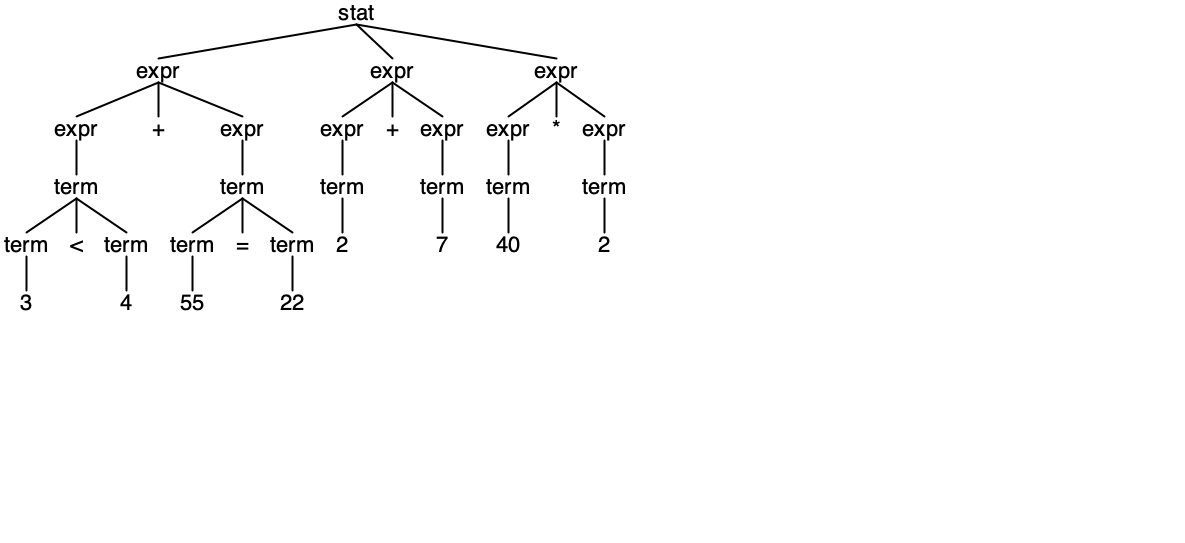
\includegraphics[width=\linewidth]{antlr4_parse_tree.png}
		\end{figure}
\end{enumerate}

%%%%%%%%%%%%%%%%%%%%%%%%%%%%%%%%%%%%%%%%%%%%%%%%%%%%%%%
%%%%%%%%%%%%%%%%%%%%%%%%%%%%%%%%%%%%%%%%%%%%%%%%%%%%%%%
% Comparison for these two versions
%%%%%%%%%%%%%%%%%%%%%%%%%%%%%%%%%%%%%%%%%%%%%%%%%%%%%%%
%%%%%%%%%%%%%%%%%%%%%%%%%%%%%%%%%%%%%%%%%%%%%%%%%%%%%%%
\section {Comparison}
\begin{itemize}
	\item For small programs, using actions will be much simpler than using the visitor pattern.
	\item Actions might be more efficient because it won't generate a parse tree. In resource-critical applications, we might not want to waste the time or memory needed to build a parse tree.
	\item The visitor pattern might be more complicated, but if the program has a large structure and you want to build a cleaner hierarchy, then it might be better to use the Antlr build-in visitor pattern, and let the intermediate class returns the object you want for future modification.
\end{itemize}
\end{document}
